\documentclass[10pt,a4paper]{article}
\usepackage[utf8]{inputenc}
\usepackage[english]{babel}
\usepackage{amsmath}
\usepackage{amsfonts}
\usepackage{amssymb}
\usepackage{graphicx}
\usepackage{mathrsfs}
\usepackage{hyperref}
\usepackage{xcolor}
\author{Francesco Corda}
\title{Data Intelligence Applications}
\setlength{\parindent}{0pt}

\begin{document}
\maketitle
\tableofcontents
\newpage
\section{DIA 2}\label{dia-2}

\subsection{Matching problems and alternating-path algorithms}\label{matching-problems-and-alternating-path-algorithms}

\subsubsection{Problem formulation}\label{problem-formulation}

\begin{itemize}
\item A \textbf{matching} is a subset of the edges of the graph such that no pair of edges share vertices.
\item A \textbf{maximal matching} is a matching that cannot be enlarged.
\item A \textbf{maximum matching} is a matching with largest cardinality.
\item A \textbf{perfect matching} is a matching in which all the vertices are matched.
\end{itemize}

Given a graph, the goal is to find a maximum matching.

\subsubsection{Alternating-paths}\label{alternating-paths}

Algorithms:

\begin{itemize}
\item Hopkroft-Karp algorithm for bipartite graphs: $O(m \sqrt n)$
\item Edmund algorithm for arbitrary graph: $O(m n^2)$
\item Micali-Vazirani algorithm for arbitrary graph: $O(m \sqrt n)$
\end{itemize}
With $m$ = number of edges, $n$ = number of nodes.

An \textbf{alternating path} is a path such that edges of the matching and edges of the complementary set alternate.

Now we consider a subset of alternating paths: an \textbf{augmenting path} is an alternating path starting and ending in unmatched vertices.

\textbf{Complementing an augmenting path} results in an alternating path whose cardinality is strictly larger than the cardinality of the initial path. In this way, we obtain a matching with a strictly larger cardinality. The new matching is found by taking the complement of the newly found augmenting path.

A matching is maximum if it does not admit any augmenting path.
\newline

Alternating-path algorithms iteratively:

\begin{itemize}
\item look for augmenting paths
\item make the complementary of them
\end{itemize}

\textcolor{red}{Until no augmenting path exists.}

\subsubsection{Looking for augmenting paths}\label{looking-for-augmenting-paths}

We are given a matching (potentially an empty matching) and we look for all the shortest augmenting paths.

Do:\\
\begin{enumerate}
\item Consider every unmatched vertex
\item Make a breadth-first search starting from every unmatched vertex
\item For every unexplored path that is not in the matching, make an expansion adding that path and the connected path in the matching if the vertex is matched
\item Label vertices as \textbf{Even} (\textcolor{blue}{blue}) and \textbf{Odd} (\textcolor{green}{green}) according to the level of the search tree, starting from Even (corresponding to Level 0)
\item If the path in the expansion contains some already visited vertex, then stop the branch and make an action according to the specific case:\\
\textbf{Case 1}: if, expanding an even node, the even node is directly connected to a vertex previously labeled as even belonging to a different subtree, then we have found an augmenting path.\\
\textbf{Case 2}: if, expanding an even node, the even node is directly connected to a vertex previously labeled as odd, then stop the search.\\
\textbf{Case 3}: if, expanding an even node, the even node is directly connected to a vertex previously labeled as even belonging to same subtree, then shrink the blossom and connect the expansion of all the node of the blossom to the vertex of the blossom.
\end{enumerate}

Case 3 in not possible in bipartite graphs, so Cases 1 and 2 are sufficient. Case 3 can happen in arbitrary graphs.

If an augmenting path is found, the blossom will be expanded.
\newline

Set of matches: $\mathscr{M} = \{(A,H), (B,G), (C, F), (D,K) \}$

Set of unmatched nodes: $\mathscr{U} = \{ E, J \}$

Frontier: $\mathscr{F} = \{ E, J \}$

\subsubsection{Weighted matching problem}\label{weighted-matching-problem}

$$ \omega_{xy} > 0 \quad \forall x,y $$

A \textbf{maximum weighted matching} is a matching with largest cardinality.


Algorithms:

\begin{itemize}
\item Hungarian algorithm for bipartite graphs: $O(n^2 m)$
\item Edmund algorithm for arbitrary graph: $O(m n^2)$
\end{itemize}

\subsubsection{Hungarian Algorithm}\label{hungarian-algorithm}

It can be implemented using two approaches:

\begin{itemize}
\item \textbf{Hungarian Algorithm using an adjacency matrix}
\begin{itemize}
\item Suitable for dense graphs
\item The algorithm returns the minimal cost matching
\item Many libraries and functions available online\\
(e.g.~scipy.optimize.linear\_sum\_assignment)
\end{itemize}
\item \textbf{Hungarian Algorithm using a graph}
\begin{itemize}
\item Suitable for sparse graphs
\item Some libraries available online (e.g.~NetworkX)
\end{itemize}
\end{itemize}

\textbf{Key ideas:}

\begin{itemize}
\item The algorithm returns the minimal cost matching
\item If a number is added to all of the entries of anyone row or column of a cost matrix, then an optimal assignment for the resulting cost matrix is also an optimal assignment for the original cost matrix
\item We can compute the maximum matching by minimizing the loss instead of the initial weights
\item If the original graph is not balanced, we can add dummy variables with the maximum cost (zero if we are maximizing) as value
\end{itemize}

\textbf{Steps:}

Given an adjacency matrix of dimension $(N \times N)$, with $N$ = number of nodes:

\begin{enumerate}
\item Subtract the smallest entry in each row from all the other entries in the row.
\item Subtract the smallest entry in each column from all the other entries in the column.
\item Draw lines through the row and columns that have the 0 entries such that the fewest lines possible are drawn.
\item If there are N lines drawn, an optimal assignment of zeros is possible and the algorithm is finished. Otherwise, go to the next step
\item Find the smallest entry not covered by any line. Subtract this entry from each row that is not crossed out, and then add it to each column that is crossed out. Then, go back to Step 3.
\end{enumerate}

\subsection{Combinatorial bandits and matching problems}\label{combinatorial-bandits-and-matching-problems}

A classical bandit problem associates unknown expected rewards to a set of candidates. A combinatorial bandit problem adds combinatorial constraints to the formulation.

\textbf{Problem formulation:}

\begin{itemize}
\item an \textbf{arm} is a candidate
\item a \textbf{superarm} is a collection of candidates
\item a \textbf{feasible superarm} is a superarm satisfying the (combinatorial constraints)
\end{itemize}

$$\mathscr{C}(\mathbf{a})= 0$$

\begin{itemize}

\item the \textbf{reward} of a superarm is the sum of the reward of the arms it contains
\item the \textbf{goal} is to maximize the cumulative, in time, expected reward
\end{itemize}

Examples of combinatorial constraints:

\begin{itemize}
\item \textbf{Knapsack}
\begin{itemize}
\item every arm has a cost
\item a superarm cannot have a cost larger than a given budget
\end{itemize}
\item \textbf{Independent set}
\begin{itemize}
\item arms are nodes of a given graph
\item a superarm cannot include arms sharing an edge
\end{itemize}
\item \textbf{Matching}
\begin{itemize}
\item arms are nodes of a given graph
\item a superarm is a matching
\end{itemize}
\end{itemize}

\subsubsection{Notation}\label{notation}

$$\begin{aligned} t &: \textsf{time} \\ A&: \textsf{set of arms} \\ a&: \textsf{arm} \\ a_t &: \textsf{arm played at t} \\ a^* &: \textsf{optimal arm} \\ X_a &: \textsf{random variable of the reward of arm } a \\ \mu_a &: \textsf{expected value of random variable } X_a \\ x_{a,t} &: \textsf{realization of random variable } X_a \textsf{ at time } T \\ x_a &: \textsf{realizations of random variable } X_a \\ \overline{x}_a &: \textsf{empirical mean of } x_a \\ n_a(t) &: \textsf{number of samples of arm } a \textsf{ at time } t \\ 2^A &: \textsf{set of superarms} \\ \mathbf{a} &: \textsf{superarm} \end{aligned}$$

\subsubsection{UCB1 (Upper Confidence Bound
1)}\label{ucb1-upper-confidence-bound-1}

\begin{itemize}
\item Every arm is associated with an upper confidence bound, providing an optimistic estimation of the reward returned by the arm.
\item At every round, the arm with the highest upper confidence bound is chosen. That is the arm that provides (optimistically) the largest expected reward.
\item After having observed the realization of the reward of the chosen arm, the upper confidence bound is updated accordingly.
\end{itemize}

\textbf{Assumptions}

\begin{itemize}

\item For simplicity, the random variable of every arm is a Bernoulli in $\{0, 1\}$ with unknown mean
\item Every arm has, potentially, a different mean
\item The model perfectly captures the scenario in which one needs to learn a conversion rate
\item In this case, the reward is given by the product between conversion rate (that is unknown) and the net margin (marginal profit, that is known)
\end{itemize}

\textbf{Pseudocode}

\begin{enumerate}
\item Play once every arm $a \in A$
\item At every time $t$ play arm $a_t$ such that
$$a_t \leftarrow \text{arg} \max_{a \in A}{\left\{ \bar{x}_a + \sqrt{\frac{2 \log(t)}{n_a (t-1)}} \right\}}$$
\end{enumerate}

The term$\sqrt{\frac{2 \log(t)}{n_a (t-1)}}$ creates the upper confidence bound. It reduces linearly as we observe new samples of the arm, and increases logarithmically as the time increases.
\newline

\textbf{General definition of Regret}

$$\mathscr{R}_{T}(\mathfrak{U}) := T\mu_{a^*} - \sum_{t=1}^{T}{\mu_{a_t}}$$

$\mathscr{R}_{T}(\mathfrak{U})$ is the expected regret after $T$

$T\mu_{a^*}$ is the expected reward of the clairvoyant optimal solution

$\sum_{t=1}^{T}{\mu_{a_t}}$ is the expected reward of the algorithm $\mathfrak{U}$
\newline

\textbf{UCB1 Regret}

$$\Delta_{a} := \mu_{a^*} - \mu_{a}$$

$$\mathscr{R}_{T} (\mathsf{UCB1}) \leq \sum_{a: \mu_{a} < \mu_{a^{*}}} \frac{4 log(T)}{\Delta_{a}} + 8 \Delta_{a}$$

The regret increases:

\begin{itemize}
\item \textbf{logarithmically} as $T$ (time) increases
\item \textbf{linearly} as $|A|$ (number of arms) increases
\end{itemize}

\subsubsection{Thompson Sampling}\label{thompson-sampling}

For every arm, we have a prior on its expected value.

In the case in which the arms rewards are Bernoulli distributions, the priors are Beta distributions. Notice that, with the opportune parameters, a Beta distribution is a uniform distribution.

For every arm, we draw a sample according to the corresponding Beta.

We choose the arm with the best sample.

We update the Beta distribution of the chosen arm according the observed realization.
\newline

\textbf{Notation}

$$\begin{aligned}
x_{a,t} &: \textsf{realizations of random variable } X_a \textsf{ at } t\\
\mathbb{P}(\mu_a = \theta_a) &: \textsf{Prior on the expected value of } X_a \\
\theta_a &: \textsf{Variable of } \mathbb{P}(\mu_a = \theta_a) \\
(\alpha_a, \beta_a) &: \textsf{Parameters of Beta distribution } \mathbb{P}(\mu_a = \theta_a)
\end{aligned}$$
\newline

\textbf{Formulas}

Beta probability distribution with parameters $(\alpha_a, \beta_a)$:

$$\mathbb{P}\left(\mu_{a}=\theta_{a}\right)=\frac{\Gamma\left(\alpha_{a}+\beta_{a}\right)}{\Gamma\left(\alpha_{a}\right) \Gamma\left(\beta_{a}\right)}\left(\theta_{a}\right)^{\alpha_{a}-1}\left(1-\theta_{a}\right)^{\beta_{a}-1}$$

$$\Gamma(n+1) := n!$$

Updating rule of the Beta distribution given a realization:

$$(\alpha_{a_t}, \beta_{a_t}) \leftarrow (\alpha_{a_t}, \beta_{a_t}) + (x_{a_t, t}, 1 - x_{a_t, t})$$
\newline

\textbf{Pseudocode}

\begin{enumerate}
\item At every time $t$, for every arm $a$
$$\tilde{\theta}_a \leftarrow \mathsf{Sample}(\mathbb{P}(\mu_a = \theta_a))$$
\item At every time $t$ play arm $a_t$ such that
$$a_t \leftarrow \text{arg} \max_{a \in A} \left\{ \tilde{\theta}_a \right\}$$
\item Update the Beta distribution of arm $a_t$ as
$$(\alpha_{a_t}, \beta_{a_t}) \leftarrow (\alpha_{a_t}, \beta_{a_t}) + (x_{a_t, t}, 1 - x_{a_t, t})$$
\end{enumerate}

\textbf{Regret}

$$\Delta_{a} := \mu_{a^{*}} - \mu_{a}$$

$$\mathscr{R}_{T}(\mathsf{TS}) \leq(1+\epsilon) \sum_{a: \mu_{a}<\mu_{a^{*}}} \frac{\Delta_{a}(\log (T)+\log (\log (T)))}{\mathscr{KL} \left(\mu_{a^{*}}, \mu_{a}\right)}+C\left(\epsilon, \mu_{a_{1}}, \ldots, \mu_{a_{|A|}}\right)$$

\begin{itemize}
\item $\epsilon$ is an arbitrarily small number
\item $\mathscr{KL} \left(\mu_{a^{*}}, \mu_{a}\right)$ is the Kullback-Leibler divergence
\item $C\left(\epsilon, \mu_{a_{1}}, \ldots, \mu_{a_{|A|}}\right)$ is a constant term
\end{itemize}

The regret increases:

\begin{itemize}
\item \textbf{logarithmically} as $T$ (time) increases
\item \textbf{linearly} as $|A|$ (number of arms) increases
\end{itemize}

\subsubsection{Combinatorial Thompson
Sampling}\label{combinatorial-thompson-sampling}

Assumptions: for simplicity, the random variable of every arm is a Bernoulli in $\{0, 1\}$ with unknown mean. For every candidate (arm), we have a Beta distribution.

The functioning is the same as the basic Thompson Sampling, except that in order to find a superarm with maximum expected reward, we need to solve a combinatorial problem.
\newline

\textbf{Pseudocode:}

\begin{enumerate}
\item At every time $t$, for every arm $a$
$$\tilde{\theta}_a \leftarrow \mathsf{Sample}(\mathbb{P}(\mu_a = \theta_a))$$
In this step, we draw one sample for each candidate from the prior distributions.
\item At every time $t$ play superarm $a_t$ such that
$$\mathbf{a}_t \leftarrow \text{arg} \max_{\mathscr{C}(\mathbf{a})= 0} \left\{ \sum_{a \in \mathbf{a}} \tilde{\theta}_a \right\}$$
In this step, we solve the associated combinatorial problem, finding a subset of arms composing the best superarm, and we pull these arms.
\item Update the Beta distribution of arm $a_t$ as
$$(\alpha_{a_t}, \beta_{a_t}) \leftarrow (\alpha_{a_t}, \beta_{a_t}) + (x_{a_t, t}, 1 - x_{a_t, t})$$
\end{enumerate}

Thompson Sampling regret:

$$\mathscr{R}_T (\mathsf{TS}) = O \left( |A| \frac{log(T)}{\Delta_{min}}\right)$$

\begin{itemize}

\item $\Delta_{min}$ is the minimum gap between the expected reward of the optimal solution and any non-optimal solution.
\end{itemize}

The regret increases:

\begin{itemize}
\item \textbf{logarithmically} as $T$ (time) increases
\item \textbf{linearly} as $|A|$ (number of arms) increases
\end{itemize}

Remember that the number of superarms is combinatorial in the number of arms.

We can't always solve the combinatorial contraints in an exact way, since it's an NP-hard problem. In many cases we use an approximate solution, that introduces an additional regret.

\subsubsection{Weighted matching problem and TS}\label{weighted-matching-problem-and-ts}

The value of every edge is a random variable, whose expected value is unknown. The problem is iterated for \textit{T} rounds.

In a matching problem, a combinatorial bandit is an algorithm that aims to learn the weights of edges.

\subsection{Online matching problems}\label{online-matching-problems}

Matching problems that are online and dynamic in time.

\textbf{Classical problem}: the input is given, the graph and the weights are completely known \textit{a priori}

\textbf{Online problem}: the graph and the weights are discovered \textit{during} time

\subsubsection{Basic bipartite online matching}\label{basic-bipartite-online-matching}

\begin{enumerate}

\item One side (left) of the bipartite graph is known a priori
\item The other side, together with the edges, is initially unknown
\item At each round, a single node enters the problem and its edges are discovered
\item At each round, either the entering node is matched with a node or it leaves the problem
\end{enumerate}

\textbf{Online inefficiency}: the online algorithm is not able to reach the value of the clairvoyant solution.

Competitive factor of an algorithm:

$$\alpha_{\mathscr{A}} = \min_{P} \frac{\Gamma_{\mathscr{A}}(P)}{\Gamma^*(P)}$$
$$\begin{aligned}\alpha_{\mathscr{A}} &: \textsf{competitive factor of the algorithm}\\
\Gamma_{\mathscr{A}}(P) &: \textsf{value provided by the algorithm}\\ \Gamma^*(P) &: \textsf{value provided by the clairvoyant algorithm}\end{aligned}$$

It's the minimization over all the problems of the ratio between the value provided by the online algorithm and the value provided by the clairvoyant algorithm. The competitive factor can't be larger than 1.

\textbf{Competitive factor and online matching}:

\begin{itemize}

\item No deterministic algorithm can have a competitive factor larger than $\frac{1}{2}$ in online bipartite matching problems
\item No randomized algorithms can have an expected competitive factor larger than $\frac{e-1}{e}$ in online bipartite matching problem
\end{itemize}

\textbf{Deterministic algorithm (greedy):} match a node with an arbitrary unmatched node. Every time a node enters the problem, we match it with an arbitrary unmatched node connected to it.

This algorithm has a competitive ratio of $\frac{1}{2}$.
\newline

\textit{Proof}:

\begin{itemize}

\item The cardinality of any maximal matching is at least $\frac{1}{2}$ of the cardinality of the maximum matching:
\begin{enumerate}
\item Be given $M^*$ (maximum matching) and $M$ (maximal matching)
\item For every edge $e = (u,v)$ in $M^*$, either $u$ or $v$ is matched in $M$ (or both), otherwise $M$ is not maximal. This is because if both these nodes were unmatched, they could be matched to increase the cardinality of the matching M.
\item So the number of matched nodes in $M$ is not smaller than the number of edges $|M^*|$, where $|M^*|$ **stand for the number of edges in $M^*$. This is a consequence of the previous statement.
\item The number of matched nodes in $M^*$ is $2|M^*|$
\item Therefore, $|M|$ is not smaller than $\frac{|M^*|}{2}$
\end{enumerate}
\item This algorithm always finds a maximal matching:
\begin{enumerate}
\item Be given M (maximal matching)
\item For every edge $e = (u,v)$ not in $M$, consider the round in which $v$ arrived
\item Either, $v$ has been matched to some node other than $u$
\item Or $v$ has not been matched since all the connected nodes (including $u$) were already been matched
\item In both cases $(u,v)$ cannot be added to $M$, not being feasible
\end{enumerate}
\end{itemize}

\textbf{Randomized algorithm (ranking):} generate randomly an ordering over the nodes that are initially available (left side), match a node with the first unmatched node in the ordering.

This algorithm has a competitive ratio of $1-\frac{1}{e}$.

\subsubsection{Generalization of online matching problems}\label{generalization-of-online-matching-problems}

Problem:

\begin{itemize}

\item the graph is discovered \textit{during} time
\item every node may wait for at most $k$ rounds before leaving
\item $k$ may be node specific (different for each node)
\end{itemize}

\textbf{Negative result}: there is no deterministic competitive algorithm even when $k$ is the same for all the nodes.

\textit{Proof, by counterexample}:

\begin{figure}[htbp]
\centering
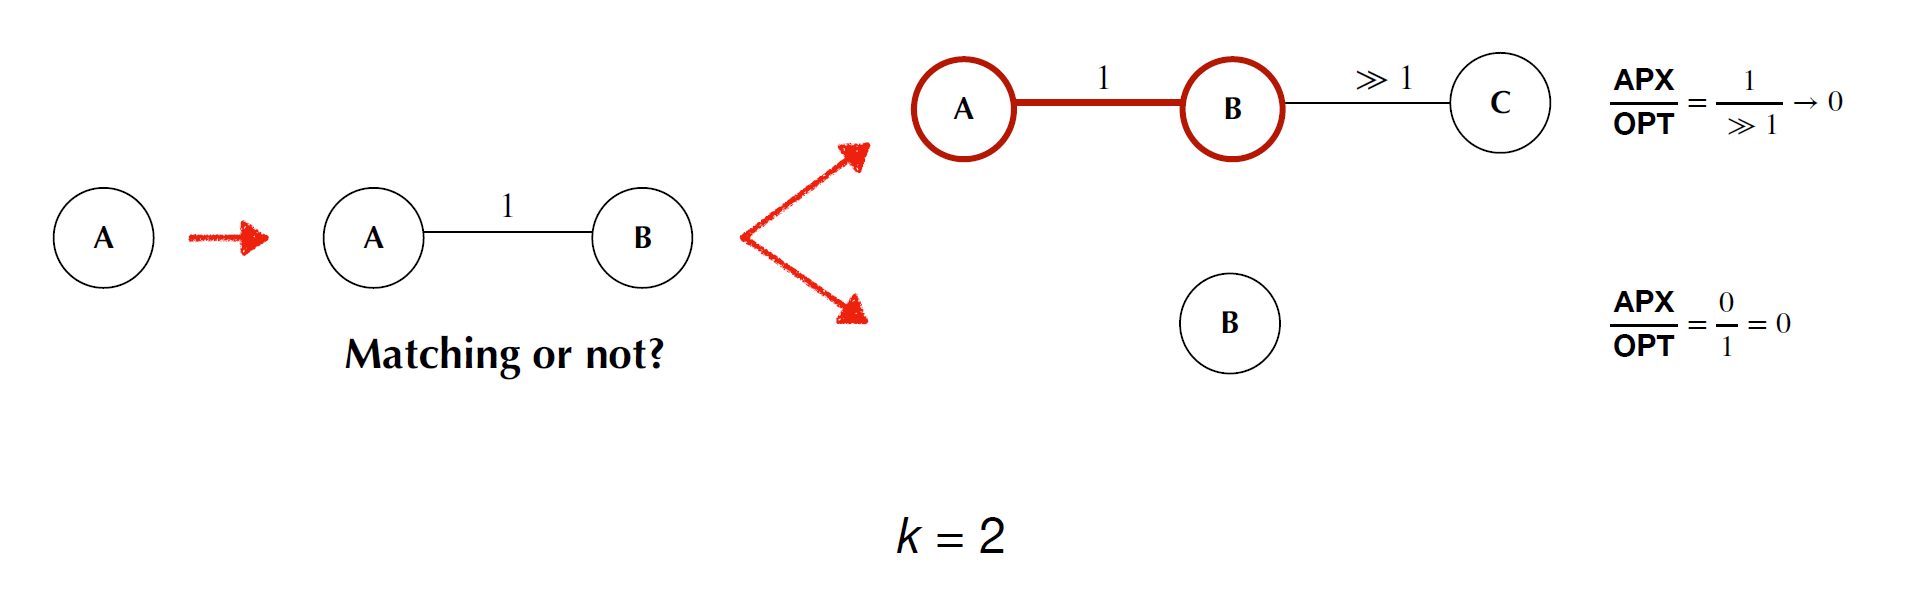
\includegraphics[width=\textwidth]{images/img_01.png}
\end{figure}

Independently on the choice that we do, we have worst case instances in which the competitive factor is 0.

\textbf{Positive result}: there is a randomized algorithm (\textbf{Postponed Dynamic Deferred Acceptance}) with an expected competitive factor of $\frac{1}{4}$ when the waiting time of every node is the same.

\subsubsection{Postponed Dynamic Deferred Acceptance}\label{postponed-dynamic-deferred-acceptance}

Every time a node $A$ enters the problem we generate two fictitious copies of the node: $A_S$ (seller) and $A_B$ (buyer). The idea behind the algorithm is to have a two-sided market.

The algorithm generates a fictitious bipartite graph in which we have the sellers on the left and the buyers on the right.

Node $B$ enters the problem in the second round. If $A$ and $B$ are connected in the original graph, then $(A_S, B_B)$ and $(B_S, A_B)$ will be connected on the bipartite graph. Two fictitious nodes associated with the same original node cannot be connected.

The next step is to find the best matching in the bipartite graph. We assume that no node is at its deadline, so it doesn't have to leave the problem. The matching is not applied until a node reaches its deadline.

In the next round, node $C$ enters the problem. We generate the fictitious nodes $C_C$ and $C_B$. We assume that in the original graph $C$ is connected to $A$ and to $B$. After the introduction of the edges, we need to find the best matching. We assume that node $A$ reaches its deadline and therefore either we match it or it will leave the problem without being matched. We select the fictitious nodes belonging to $A =(A_S, A_B)$ and the buyer node matched to $A_S$ in the optimal matching, in this case $B_B$.

The node $A$ is not labeled yet. In the case the critical node (the node at the deadline) has no label, we decide randomly with a probability of $\frac{1}{2}$ its label between seller and buyer.

If the realization is seller, we assign the label seller to it. Node $B$ is then labeled as buyer, since it was matched to $A$ in the bipartite graph. We match $A_S$ and $B_B$ and remove the fictitious nodes $A$ and $B$ from the problem.

If the realization for $A$ is instead buyer, we assign the seller label to $B$ (since it was match to $A_S$). In this case we remove $A$ from the graph, without matching with $B$.

Suppose that no other nodes enter the problem and node $B$ reaches its deadline. We now have a label already assigned to it, so we don't have to draw randomly. We label node $C$ according to the previous labels and remove the fictitious nodes.

When a node is at its deadline:
\begin{itemize}
\item if it's labeled as seller, we \textbf{match} it
\item if it's labeled as buyer, we \textbf{discard} it
\end{itemize}

When we remove a node from the graph, we need to remove both buyer and seller nodes, because they are a representation of the same node in the problem.

\textbf{Worst-case example showed before}

The algorithm returns a matching with a value $>>1$ with a probability of $\frac{1}{2}$.

The competitive factor in the worst case example seen before is about $\frac{1}{2}$, both in the case in which node $C$ enters the problem and in the case in which it doesn't.

\section{DIA 4}\label{dia-4}

\subsection{Information cascades}\label{information-cascades}

\subsubsection{Model}\label{model}

We have a set of users. Each of them can choose an action within a set. We assume for semplicity to have two actions, labeled $1$ and $0$.

Users do not know which action is the best, initially the two actions are equally valuable.

At the begininning, each user receives a signal that an action is better than the other with a probability $p > \frac{1}{2}$ and updates their belief.

For instance, assume that the first user receives a signal that action $1$ is better than action $0$: this means that the first user believes that $1$ is better than $0$ with probability $p$.

\textit{Consider the following example.}

Assume that the received signals are the following:
\begin{enumerate}
\item $1$ is better than $0$ with probability $p$
\item $0$ is better than $1$ with probability $p$
\item $1$ is better than $0$ with probability $p$
\item $1$ is better than $0$ with probability $p$
\item $1$ is better than $0$ with probability $p$
\end{enumerate}

Each user can observe the actions of the previous user and update their beliefs accordingly.

If many users previously selected the same action, then the next user will update its belief accordingly.

The belief of the first user depends only on the received signal, therefore the action selected will be $1$.

The other users observe that the first user selected action $1$. This means that the first user received a signal that $1$ is better than $0$. The second user updates her belief accordingly: now actions $1$ and $0$ have the same probability to be the best.

The new belief of the second user is: $0$ and $1$ are equally valuable. We assume that ties are broken in favor of the received signal, so the second user selects $0$.

The next users update their beliefs.

Ther third, fourth and fifth users select action $1$.

\textit{Consider the following example.}

The first 3 users selected action 1 and the signal received by the fourth and fifth users are:

\begin{enumerate}
\setcounter{enumi}{3}
\item $0$ is better than $1$ with probability $p$
\item $0$ is better than $1$ with probability $p$
\end{enumerate}

The fourth user will select $1$ even if her signal tells that $0$ is better. This is because a $0$ and a $1$ nullify each other, but two $1$s win against a $0$.

The same holds for the last user.

\textit{Consider the following example}.

The first two users chosed action $1$. This happens if both users received a signal that $1$ is better than $0$. Then we have a large number (7) of users that received a signal that $0$ is better than $1$.

The third user will select $1$ even if her signal tells that $0$ is better. The same for all the other users.

Technically speaking: the first two users, selecting $1$, generated an \textbf{information cascade} since, after them, all the users select $1$ regardless their prior.

\subsubsection{Cascade activation}\label{cascade-activation}

On the horizontal axis, we have users/time. On the vertical axis we have the number of times the users selected $1$ minus the number of times the users selected $0$.

Until the difference $\#1 - \#0 \le 1$, the actions chosen by the users \textit{depend on the prior}.

Otherwise we have a cascade, meaning that the actions chosen by the users \textit{do not depend on the prior}.

\subsubsection{Cascade activation probability}\label{cascade-activation-probability}

Assume that the prior is $P(1)=q$ and $P(0)=1-q$.

The probability of a cascade is \textit{larger than} the probability $\bar{p}$ to have $3$ consecutive $1$-signals or $0$-signals:
$$\bar{p} = q^3 + (1 - q)^3$$

This is a stronger than necessary condition, because it would be sufficient to have the first two users with the same signal to generate a cascade.

The probability of a cascade tends to 1:
$1-(1-\bar{p})^{\frac{T}{3}} \xrightarrow[T\rightarrow \infty]{} 1$

Again, this probability is smaller than the actual probability of a cascade, but it still tends to $1$.

\subsubsection{Mathematics}\label{mathematics}

\textbf{Prior:}
$$\mathbb{P}[1>0] =\mathbb{P}[0>1]=\frac{1}{2}$$

The probability that one action is better than another is $\frac{1}{2}$, meaning that the best is chosen by chance.

\textbf{One Signal:}

$$\begin{aligned}
&\mathbb{P}[\{1\} \mid 1>0] =\mathbb{P}[\{0\} \mid 0>1]=p>\frac{1}{2} \\
&\mathbb{P}[\{0\} \mid 1>0] =\mathbb{P}[\{1\} \mid 0>1]=1-p<\frac{1}{2} \\
\end{aligned}$$

$\{\cdot\}$ is the notation for the signal

The probability to receive a signal given the action preference is greater than $\frac{1}{2}$ if it is in accordance with the action preference order, smaller otherwise.

\textbf{Remarks:}

Bayes Rule:
$$\mathbb{P}(A|B) = \frac{\mathbb{P}(B|A)\mathbb{P}(A)}{\mathbb{P}(B)}$$

Law of Total Probability:
$$\mathbb{P}(A) = \sum_{n}{\mathbb{P}(A|B_{n})\mathbb{P}(B_{n})}$$

\textbf{Bayes Rule application:}

$$\begin{aligned}
\mathbb{P}[1>0 |\{1\}] &=\frac{\mathbb{P}[\{1\} | 1>0] \mathbb{P}[1>0]}{\mathbb{P}[\{1\} | 1>0] \mathbb{P}[1>0]+\mathbb{P}[\{1\} | 0>1] \mathbb{P}[0>1]}= \\
&=\frac{p \frac{1}{2}}{p \frac{1}{2} + (1-p) \frac{1}{2}}=p
\end{aligned}$$

The probability of the action preference order given the received signal is equal to the probability of receiving that signal given the precedence order.
\newline

\textbf{Two signals:}

$$\mathbb{P}[\{0,1\} \mid 1>0]=\mathbb{P}[\{0\} \mid 1>0] \mathbb{P}[\{1\} \mid 1>0]=p(1-p)$$
\newline

\textbf{Bayes Rule application:}

$$\begin{aligned}
\mathbb{P}[1>0 |\{0,1\}]&=\frac{\mathbb{P}[\{0,1\} | 1>0] \mathbb{P}[1>0]}{\mathbb{P}[\{0,1\} | 1>0] \mathbb{P}[1>0]+\mathbb{P}[\{0,1\}| 0>1] \mathbb{P}[0>1]}= \\
&=\frac{p(1-p) \frac{1}{2}}{p(1-p) \frac{1}{2}+p(1-p) \frac{1}{2}}=\frac{1}{2}
\end{aligned}$$

Generic number of signals:

$$\begin{aligned}
\mathbb{P}\left[1>0 \mid\left(n_{0}, n_{1}\right)\right] &=\frac{\mathbb{P}\left[\left(n_{0}, n_{1}\right) \mid 1>0\right] \mathbb{P}[1>0]}{\mathbb{P}\left[\left(n_{0}, n_{1}\right) \mid 1>0\right] \mathbb{P}[1>0]+\mathbb{P}\left[\left(n_{0}, n_{1}\right) \mid 0>1\right] \mathbb{P}[0>1]}= \\
&=\frac{p^{n_{1}}(1-p)^{n_{0}} \frac{1}{2}}{p^{n_{1}}(1-p)^{n_{0}} \frac{1}{2}+p^{n_{0}}(1-p)^{n_{1}} \frac{1}{2}}= \\
&\textsf{Under the assumption: } \Delta=n_{1}-n_{0}>0 \\ &=\frac{p^{\Delta}p^{n_{0}}(1-p)^{n_{0}} \frac{1}{2}}{p^{\Delta}p^{n_{0}}(1-p)^{n_{0}} \frac{1}{2}+p^{n_{0}}(1-p)^{n_{0}}(1-p)^{\Delta} \frac{1}{2}}= \\
&=\frac{p^{\Delta} \frac{1}{2}}{p^{\Delta} \frac{1}{2}+(1-p)^{\Delta} \frac{1}{2}}=\frac{p^{\Delta}}{p^{\Delta}+(1-p)^{\Delta}}=\frac{1}{1+\frac{(1-p)^{\Delta}}{p^{\Delta}}}>\frac{1}{2}
\end{aligned}$$

$(n_0, n_1)$ is a signal composed of $n_0$ signals $0$ and $n_1$ signals $1$

\subsubsection{Model refinements}\label{model-refinements}

\begin{itemize}
\item Multiple actions
\item Different priors
\item Non-uniform signals
\item Users with different preferences
\end{itemize}

\subsubsection{Considerations}\label{considerations}

In principle, a manipulator could always start a cascade by introducing, e.g., fake reviews.

In the case of advisor applications, the possibility to rate the reviews is crucial to block adversarial cascade.

\subsection{Direct Effects}\label{direct-effects}

We consider \textit{social influence phenomenones}, in which users have a complex knowledge of the possible actions, but the utilities (the value) that they obtain taking the actions strictly depend on the action chosen by the neighbors in the social network.

We represent a social network in a classical way, using a graph, where nodes represent users, edges represent the connections between pair of users. We assume that the edges are direct, since given a pair of users, the ways a user affect the others may be different.

\subsubsection{Independent Cascade
Model}\label{independent-cascade-model}

Each edge is associated with a parameter $p_{a,b}$, where $a$ and $b$ are nodes, that represents how node $a$ affects node $b$. This model is called \textbf{independent cascade} and it is common in the scientific literature. Usually, the parameters $P_{x,y} \in [0,1]$. $P_{x,y}$ is interpreted as the probability with which node $a$ affects node $b$.

\begin{itemize}
\item Every node (user) is in one of a set of states
\begin{itemize}
\item Basic model: states in $\{susceptible, active, inactive\}$. A \textit{susceptible} node is a node that can be activated by the influence of some neighbor, an \textit{active} node is a node that has been activated by a neighbor, an \textit{inactive} node is a node that has been previously activated.
\end{itemize}
\item Time is discrete
\item If node $a$ becomes active at time $t$, then at time $t+1$ it can activate neighbour $b$ with probability $p_{a,b}$
\item If node $b$ does not activate at $t+1$, then node $a$ cannot activate node $b$ in future
\item If a node activates at $t$, then at $t+1$ it will become inactive
\end{itemize}

Basically, once a node activates he can activate the neighbors, but it cannot do the same in future time points.

\subsubsection{Seeding}\label{seeding}

We consider the possibility to buy a subset of nodes, called \textbf{seeds}, to generate a cascade of influence that affects the other nodes. The idea is that a seed could activate some nodes, that will do the same with the neighbors, generating a cascade.

\begin{itemize}
\item A subset of nodes are seeds
\item The seeds are active nodes that try to influence the neighbours
\item In principle, a social influencer buys a subset of nodes that will be the seed
\end{itemize}

\textbf{Example}

The \textit{susceptible} nodes are in blue, the \textit{seeds} in green, the
\textit{active} node in red and the \textit{inactive} nodes in gray. Suppose that the node $a$ is the seed, suppose that the edges connecting $a$ to $b$ an $a$ to $g$ activate. Remember that there is a given probability that they will activate, in this case we assume that only these two edges activate. The idea is that we are randomly drawing the fact that an edge activates or not, given the probability associated with the edge. Nodes $b$ and $g$ activate due to the edge, then the edges connecting $b$ to $c$ and $g$ to $d$ activate. As a result nodes $c$ and $d$ activate, while nodes $b$ and $g$ become inactive. Then the edges connecting $d$ to $c$ and $c$ to $e$ activate. Thus, node $e$ activates while node $c$ and $b$ become inactive. Finally we suppose that the edge connecting $e$ to $f$ activates and so the node have activated. In general we have that not all the network is activated due to a cascade, but probably only a small portion of the network.

We can provide an alternative interpretation of the model. We can imagine that at the beginning, for every possible edge we draw whether it is active or not. In the slide we reported active edges. Reporting only the direct edges that are activated, we have a graph composed only of red edges in this case, called \textbf{live-edge graph}. Every node that can be reached by some seed in the live-edge graph will activate.

\subsubsection{Linear Threshold Model}\label{linear-threshold-model}

We consider a different model called \textbf{linear threshold.} The edges are associated with a parameter $w_{x,y} \in [0,1]$. The meaning is similar to the independent cascade case, even if the uses are different. The nodes are associated with a parameter $\theta \in [0,1]$ called \textbf{threshold}. For every node$\sum_{y}{w_{x,y} \le 1}$.

\subsubsection{Activation}\label{activation}

The peculiarities of the linear threshold model is that:

\begin{itemize}
\item once active, a node keeps to be active
\item a node activates if it holds $\sum_{y: y \text{ is active}}{w_{y,x} \ge \theta_{x}}$
\end{itemize}

So differently from the dependent cascade the node does not become inactive after its activation and has the possibility to influence the neighbors in the future. A node activates if the sum of the parameters $w$ of the edges coming to that node from active nodes is larger than its threshold.

Here an example. The number reported inside the node is the threshold $\theta$. Suppose that we have only one seed and it is the node $a$. Node $b$ cannot activate since the sum of the incoming weights is smaller than its threshold. The same holds for node $d$. Instead the threshold of node $g$ is smaller than the incoming weight, that is the edge connecting $a$ to $g$ has a weight of $0.2$ while the threshold of node $g$ has a value of $0.1$. Node $g$ activates. The activation of node $g$ leads to the activation of the edges leaving node $g$. We don't activate the edge connecting $g$ to $a$ just because node $a$ is already active, but in principle this edge activates.

Now, node $d$ can activate since the sum of the incoming weights is larger than his threshold (that is $0.3$), while the sum of the weights is $0.1$ for the edge connecting $a$ to $d$ and $0.2$ for the edge connecting $g$ to $d$. Instead node $e$ cannot activate because the threshold is $0.6$ and the edge connecting $g$ to $e$ is $0.2$.

The activation of node $d$ leads to the activation of the edges leaving that node. Now we have that node $b$ can activate since the sum of the incoming weights is $0.7$ while the threshold is $0.6$. Also node $e$ now can activate.

Here the result. We can activate the edges living nodes $b$ and $e$ and now node $c$ can activate given that the threshold is $0.7$, while the incoming weight is $0.9$.

\subsubsection{Extensions}\label{extensions}

\begin{itemize}
\item \textbf{Contextual problems:} this holds for independent cascade and linear threshold models. The probabilities associated with the edges depend on the messages (usually, features are used to characterize the messages). We could imagine a number of classes of messages. This classes could be characterized for instance in terms of features. For each class of message we could have different probabilities or weights. For instance consider a pair of nodes: the second node could be activated by political messages sent by the first node, but not by other kinds of messages.
\item \textbf{Negative effects:} active/inactive nodes can change the state, returning to susceptible, due to the negative influence of another node (usually, edges can provide either a positive or negative influence). For instance a node could like a post, but since another node also likes that post, then the first changes opinion and does not like the post anymore.
\end{itemize}

\subsection{Influence maximization}\label{influence-maximization}

We define the problem of \textbf{influence maximization} and discuss its solution. We consider only the independent cascade model. A similar approach can be followed for the linear threshold case.

\textbf{Inputs:}
\begin{itemize}
\item Network
\item Influence probabilities
\item Budget (in terms of number of nodes), the number of nodes that we can buy
\end{itemize}

\textbf{Actions:}
\begin{itemize}
\item Subset of nodes (seeds) to select simultaneously with cardinality not larger than the budget. These nodes will be the seeds that we place in the network.
\end{itemize}

\textbf{Goal:}
\begin{itemize}
\item Maximization of the expected number of the active nodes at the end of the cascade
\end{itemize}

The problem is to find the best subset of nodes, subject to a budget constraint, to maximize the expected number of nodes that have been activated during the cascade.

Consider the example. We select some possible seeds, for instance nodes $a$ and node $f$. Now, the crucial issue is to compute the activation probabilities of the nodes, that is the probability with which each node will activate, given that we place the two seeds.

This task is not straightforward in general, in this case the task is easy and in particular the probability that node $a$ activates is $0.3$ because it is just given by the probability of the edge connecting $g$ to $a$ and the probability that node $b$ activate is just $0.06$ since it is given by the product between $0.3$ and
$0.5$. In general with arbitrary graph the task is a bit involved.

\subsubsection{General case}\label{general-case}

\begin{enumerate}
\item Call $E$ the set of $m$ edges $\{e_1, e_2, \ldots, e_m \}$. Call $x = (x_1, x_2, \ldots, x_m)$ a binary vector such that $x_i = 1$ if edge $e_i$ is present and $0$ otherwise.
\item Notice that every $x$ corresponds to a live-edge graph because we are drawing a sample for every edge and we are generating the corresponding live-edge graph.
\item In this algorithm we need to enumerate every $x$ (every live-edge graph), there are $2^m$ of them. In practice the enumeration can be done by using an enumeration tree with a branching factor of $2$, where at each level of the tree we are considering a single $x_i$. For instance the left branch of the tree corresponds to assigning $0$ to a given $x_i$, while the right branch corresponds to assigning $1$ to that variable. This enumeration tree could be visited by using depth-first strategy in order to have memory occupancy that is linear in the number of nodes.
\item For every $x$ check whether there is a path connecting a node with some seed.
\item For every $x$ compute the corresponding probability, that is the probability that this live-edge graph occurs. The probability of the live-edge graph is given by the product of all the probabilities, that is $p$ in the case of the edges that have been activated and $1-p$ in the case of the edges that didn't activate.
\end{enumerate}

The activation probability of a node is the sum of the probabilities of the live-edge graphs with a path connecting the node with some seed.

To summarize we need to enumerate all the possible live-edge graphs and have them in a table, for instance we denote them with $G_1, G_2, G_3, \ldots, G_K$. For every live-edge graph we need to find a set of nodes that have been activated during the cascade and the corresponding probability of the graph. Given this table we can calculate the expected number of activated nodes given the initial set of seeds and in addition we can calculate the probability that each single node will activate for some possible cascade.

\subsubsection{Computational considerations}\label{computational-considerations}

\begin{itemize}

\item The computation of the activation probabilities associated with each node is impractical, requiring exponential time in the number of the edges, specifically $2^{|E|}$.
\item We can approximate these probabilities by using Monte Carlo sampling. This approximation can be arbitrarily good and can be done in polynomial time.
\end{itemize}

We approximate the calculation of the activation probabilities by means of Monte Carlo sampling technique.

\subsubsection{Monte Carlo sampling}\label{monte-carlo-sampling}

\begin{enumerate}
\item For every node $i$ assign $z_i = 0$, these variables count the number of Monte Carlo simulations in which a node has been activate
\item Randomly generate a live-edge graph according to the probability of every edge
\item For every node that is active due to the generated live-edge graph, assign $z_i = z_i + 1$
\item Go to Step 1 unless $k$ repetitions have been done
\item For every node return $\frac{z_i}{k}$, that is the frequency with which the node has been activated in our simulation Monte Carlo simulation
\end{enumerate}

Checking whether a node has been activated in the simulation can be done by using a breadth-first search excluding nodes previously visited. Since there will be multiple seeds we need that our search has multiple rootes and we are basically doing a breadth-first search, starting from multiple rootes and then going down the tree.

In the case of Monte Carlo sampling the table reported in the slides present some differences with respect to the table in which we completely enumerate all the live-edge graphs. First, the live-edge graphs are not generated by enumeration, but they are drawn from the probability distributions. This means that some live-edge graphs may be not present in the table as well as some live-edge graphs may be present multiple times. The fact that they are present multiple times in some way is simulating that their probability of occurring is larger. Second, we don't need the calculation of the probabilities anymore.

\subsubsection{How many repetitions?}\label{how-many-repetitions}

With probability of at least $1-\delta$, the estimated activation probability of every node is subject to an additive error of $\pm \epsilon n$ when the number of repetitions is
$$R = O\left(\frac{1}{\epsilon^2} \log{\left(|S|\right)} \log{\left(\frac{1}{\delta}\right)}\right)$$

$n =$ number of nodes, $S=$ set of seeds.

Notice that, if we want to have a additive error that does not depend on the number of nodes, we need to set $\epsilon$ as a function how $\frac{1}{n}$, and this means that the number of repetitions that we need depends on the square of the number of nodes.

\subsubsection{IM exact solution}\label{im-exact-solution}

\begin{itemize}

\item The influence maximization problem cannot be solved exactly in polynomial time, even accepting to use Monte Carlo sampling to approximate the influence.
\item Every exact algorithm requires exponential time, the problem is proved to be NP-hard.
\item The basic exact algorithm enumerates all the possible subsets of $k$ nodes (the seeds), for every subset it evaluates the expected number of active nodes.
\end{itemize}

Finally, the algorithms selects the best solution among all the enumerated ones.

\subsubsection{Approximating IM}\label{approximating-im}

Influence maximization admits a greedy algorithm, providing a constant approximation. The problem is sub-modular and a simple greedy algorithm guarantees an approximation ratio of about $0.63$.

\begin{itemize}
\item A simple greedy algorithm provides a constant approximation of
$$1-\frac{1}{e} \simeq 0.63$$
\item The algorithm works as follows:
\begin{itemize}
\item For every node that is not a seed, evaluate the marginal increase in the objective function if that node were a seed
\item Select the node for which the marginal increase is maximised and add it to the set of seed
\end{itemize}
\end{itemize}

The algorithm is repeated until there is remaining budget, so we can buy new seeds.

\subsubsection{Considerations}\label{considerations-1}

The approximation bound follows from the sub-modularity property

$$\forall X \subseteq Y, x \notin Y: f(X \cup \{x\}) - f(X) \ge f(Y \cup \{x\}) - f(Y)$$

\textbf{Interpretation:} adding a seed to a set of seeds gives a marginal increase in the utility function larger than adding the same node to a strictly larger set of seeds.

The greedy algorithm works incrementally, adding seed by seed, however this incremental process is not simulating that the nodes become seeds incrementally (we select a seed, we observe the result and then we select another seed). Once the algorithm has chosen the set of seeds, they become seeds simultaneously. The fact that the algorithm works incrementally is used only to decide a set of seeds, not not to apply the seeds one by one, observing the result of the cascade of the first, then the second and so on.

\subsubsection{Model generalization}\label{model-generalization}

\begin{itemize}

\item Each seed requires a different cost in terms of monetary resources. In this case the budget is expressed in terms of monetary resources and every node can have a different weight. In the objective function the goal would be not to maximize the number of nodes that are being activated, but the number of activated nodes multiplied by the weight of each possible node.
\item The budget is expressed in monetary resources
\item Every node can have a different weight
\item The greedy algorithm maximises the marginal increase in utility normalized by the cost of the seed and it can be used also in this case obtaining the same theoretical guarantees that we have in the general mode
\end{itemize}

\subsection{Learning issues in influence maximization}\label{learning-issues-in-influence-maximization}

We focus on the situation in which some information on the social network is not known and we need to earn it \textit{online}.

Initially we consider a social network and an uncertainty situation. In particular, the most common case studied is when the network is known (that is the nodes and the edges) but the probabilities associated with edges are unknown. So the idea is that our problem is repeated in time. We have a budget $B$ used to select a subset of seeds and then we observe the cascade. Once the cascade is concluded, we observe the nodes that have been activated and we have again a budget $B$ to spend to select a potentially different set of seeds in time. We can exploit the observation that we collect at each repetition of all the problems to update the estimates about the probabilities associated with edges. We use these probabilities when we select a new set of seeds at the new repetition of the problem.
\newline

\textbf{Three learning scenarios}

\begin{itemize}

\item We can observe the activation of all the edges
\item We can observe the activation of a small portion of the edges
\item We can observe only the activation of the nodes
\end{itemize}

\subsubsection{Fully observable edges}\label{fully-observable-edges}

It is possible only when we can observe directly the edge. This happens for instance in the case of a retweet on Twitter: we can observe the node that has been activated and the node that activated it.

The case in which all the edges can be completely observed is an easy problem, because it can be addressed as a standard combinatorial multi-armed bandit problem.
\newline

\textbf{Standard Combinatorial MAB problem}

\begin{itemize}

\item Every edge is a Bernoulli random variable whose expected value is unknown.
\item For every edge we can draw a sample from a Beta distribution (adopting a TS approach) or use an upper confidence bound (adopting a UCB1  approach).
\item Once we have a value for every edge, we use the greedy algorithm to find the optimal solution, or an approximate solution with a given approximation bound.
\end{itemize}

\subsubsection{Partially observable edges}\label{partially-observable-edges}

The second scenario is when we can only observe a small portion of the edges and we want to use this information to infer about all the possible edges of the network. This is also motivated by the fact that a cascade due to a seed involves usually a small ratio of the nodes with respect to all the possible nodes in the network. So we need many repetitions of the problem in order to collect a sufficient number of samples.

\begin{itemize}

\item When the network is huge, collecting a sufficient number of samples for each edge is impossible
\item Usually, the cascade due to a seed involves a small ratio of the nodes
\end{itemize}

In this case the goal is to reuse the observations that we collected in some part of network for another part of the network.
\newline

\textbf{Idea}

\begin{itemize}

\item We exploit the information on the observable edges to infer the probabilities of the non-observable edges
\item This requires assuming some structure about the probabilities of the edges, in other words the edges cannot have every possible probability
\item \textbf{Features} $\mathscr{F} = \{1,2,\ldots,l\}$
\item \textbf{Values of the features} $x_{i,j} \in [0,1]$ $i$ is the edge, $j$ is the feature. If the value is equal or close to $1$  this feature is very important for the edge, instead if this value is close to zero, this feature has no importance as an effect for this edge
\item \textbf{Parameters of the features} $\theta_j \in [0,1]$, $j$ is the feature
\item \textbf{Linear dependency} $p_i = \sum_{j=1}^{l}{\theta_j x_{i,j}}$, the probability of an edge is given by a linear combination of the feature
\end{itemize}

\textbf{Example:} if we interpret the features as interests of the users, a value of $1$ means that both users share that interest, instead a value of $0$ means that this pair of users doesn't share that interest.

\subsubsection{Algorithm rationale}\label{algorithm-rationale}

The parameters of the features are estimated by using linear regression

\begin{itemize}
\item (While the values of the features for every edge are known)
\item Given the values of the probabilities a UCB1-like term is added to obtain an upper bound
\item The optimization is performed with the use of the greedy algorithm, by repeating the problem for a long time. Since we are using a specific  upper bound for the problem we have that the regret will go to $0$.
\end{itemize}

\subsubsection{Non-observable edges}\label{non-observable-edges}

We only observe the activation of the nodes, without observing the activation of the edges.

We need to observe the evolution of the cascade. At any time point of the cascade, we take trace of the active nodes.

If multiple nodes could have caused the activation of a node, maximum likelihood techniques are used to estimate which is the edge that most likely activated the node. Usually, maximum likelihood techniques do not scale well with the number of neighbours ($20$ nodes is already a huge number). In that case alternative techniques (usually frequentist techniques) should be used.

\subsection{Laboratory}\label{laboratory}

\subsubsection{Credit assignment}\label{credit-assignment}

$$p_{vw} = \frac{\sum{credit_{uv}}}{A_{v}}$$

$$credit_{uv} = \frac{1}{\sum_{w \in S}}{I(t_{w} = t_{v} - 1)}$$

\subsubsection{LinearUCB}\label{linearucb}

When the arms space is huge, we can exploit the information gained on observed arms to estimate the reward function of non-observed arms.
\newline

\textbf{Linear Environment}

\begin{itemize}

\item Each arm $j$ is associated with a feature vector $x_{j} = (x_{j1}, x_{j2}, x_{j3}, \ldots, x_{jD})$ with $x_{ji} \in [0,1]$
\item The rewards is a linear combination of the arm feature vector and a parameters vector $\theta$: $r_t = x_t^T \theta$
\end{itemize}

\textbf{Pseudocode:}
\begin{itemize}
\item \textbf{Input:} set of arms $A$, parameter $c>0$
\item \textbf{Initialization:} $B_0 = 0 \in R^D, M_0 = I \in R^{d \times d}$
\end{itemize}
for $t=1, 2, \ldots, n$ do
\begin{enumerate}
\item $\theta_{t-1} = M_{t-1}^{-1} B_{t-1}a$\\
$\mathsf{UCBs} = x^T \theta_{t-1} + c \sqrt{x^T M_{t-1}^{-1} x}$
\item Choose the arm with maximum UCB value
\item Update matrices:
\begin{enumerate}
\item $M_t = M_{t-1}, B_t = B_{t-1}$
\item $M_t = M_t + x_t x_t^T$ and $B_t = B_t + x_t r_t$
\end{enumerate}
\end{enumerate}

\subsubsection{IMLinUCB}\label{imlinucb}

Wen et al. ``\href{https://dl.acm.org/doi/10.5555/3294996.3295062}{\textbf{Online influence maximization under independent cascade model with semi-bandit feedback.}}'' \textit{Advances in neural information processing systems, 2017.}

\end{document}